\subsection{Spectroscopy}

When an electron hole pair is recombining, the energy is released as a photon. By measuring this photon in a photo detector it can be determined how much energy that was released during recombination. This energy tells how large the bandgap is, which in turn tells us something about the material. By shining light with high enough energy and intensity on to a sample, the light will excite electrons into all available states. When these states recombine, the emitted light can be detected by a camera as a spectra of different wavelengths. The indirect bandgap for silicon is just around 1.1~eV. This result in the energy 1.1~eV for the emitted photons. If there are impurities or defects in the silicon crystal, they can in turn emit light at different photon energies.

\begin{figure}[H]
\centering
%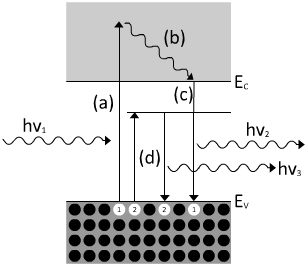
\includegraphics[width=10cm,bb=0 0 306 265]{luminisence.png}%
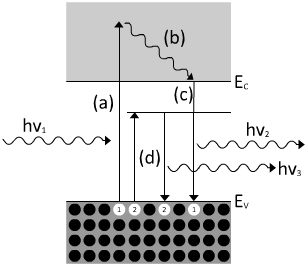
\includegraphics[width=10cm]{luminisence}%
\caption{Eksitation og recombination}%
\label{fig:luminescence}% 
\end{figure}

Figure \ref{fig:luminescence} show incoming light with high intensity in a direct bandgap material. In $a$, an electron is excited to a high energy state, which falls down to a lower energy state in $b$, after a very short time. When this electron recombines in $c$, it emits a photon with energy equal to $E_c$. Another electron is excited in $d$, which reach a so-called trap state, which can occur from impurities in the crystal, or defects. This trap state have a lower energy than the bandgap, and when this electron hole pair recombines, and lower energy is emitted. By looking at the light from such trap states, certain known spectra related to different impurities and defects can be recognized.

\subsection{Spectrometer}

In order to analyze different wavelengths, they need to be separated, and detected individually. This is done in a spectrometer. By shining light on a diffraction grating, the light is reflected at different angles by

\begin{equation}
d\sin(\theta _m)=m\lambda
\label{eq:grating_equation}
\end{equation}

where $d$ is the distance between the grating lines, $\theta _m$ is the outgoing angel of the light, $m$ is an integer denoting the diffraction order, and $\lambda$ is the wavelength. For large wavelength resolution, the angle of the reflected light will be large as well. So, in order to measure a large specter of wavelengths, several measurements with different center wavelengths is needed. This is due to physical limitations regarding the photo detector. There is a limit to how small a single pixel can be, and how long the array of pixels you can fit in the system. Each pixel translate to a separate wavelength, which measure the intensity of that wavelength only, which result in a full spectra of wavelengths and intensities. 

\subsection{Noise}

In addition to the actual photoluminescence signal, there will be noise. Noise can be from stray light in the surrounding environment hitting the camera, or it can noise from the electronics in the camera itself. Examples of noise are thermal noise, dark current, uneven amplification for different pixels in the detector, second (or more) order diffracted light from other wavelengths, background noise and different intensities for different photon energies. All measurements will be subject to noise. By having a longer integration time the signal to noise ratio is likely to increase. But a long integration time, result it a higher dark current signal. Dark current is thermally generated in the detector of the camera, and is independent of the incoming light. By cooling down the detector, the dark current noise is reduced to a minimum. This in turn makes long integration time possible, without the noise floor drowning weak signals. By blocking the signal, the dark current in addition to background noise can be measures, and then subtract this noise from the measurement containing the signal. Background noise should be fairly static, compared to dark current, and can be subtracted accurately. As for dark current, only an averaging is possible to subtract. This remaining white noise component is not possible to remove, and is clearly visible in areas without any signal. Second order diffraction can be a problem when pumping with a laser due to high intensities. Using a 532~nm laser to pump with, can result in second order diffraction at 1064~nm, which corresponds to 1.165~eV. The laser is reflected off the sample, and needs to be blocked before entering the spectrometer. However, it is possible that some light may slip through the filter, and with 532~nm pumping wavelength, the second order diffraction energy is right next to silicon bandgap which is actual signal from the photoluminescence. By using a different pumping wavelength, or having a close to perfect filter would solve this problem.